\chapter{Ferramenta análise de elementos regulatórios} \label{cap2}

Dentro do conjunto de métodos para busca de elementos regulatórios, foram selecionados os métodos que obtém melhores resultados na identificação de elementos regulatórios e que focam as buscas em genes co-regulados, uma vez que, em busca em genes ortólogos, para fazer a análise computacional é necessário as sequências das espécies relacionadas em uma mesma árvore filogenética, entretanto como muitos organismos ainda não tiveram o genoma decodificado, a árvore filogenética ficaria incompleta, prejudicando a análise. A seguir é detalhado teoricamente cada algoritmo implementado, então é explicado a implementação da ferramenta de analise de elementos regulatórios que está sendo implementada.
 
\section{Median String}

\cite{Jones2004book} descreve o \textit{Median String Problem} apresentando ele como um algoritmo simples mas eficiente em suas buscas, entretanto a quantidade de elementos regulatórios que ele encontra é muito pequena, identificando apenas elementos regulatórios muito conservados. Este algoritmo foi estudado e implementado para ter um entendimento básico de  algoritmos utilizados para busca de elementos regulatórios.

Para fazer as buscas de elementos regulatórios, o algoritmo procura por uma palavra média em todas as sequências de DNA, com o menor número de mutações,os números de mutações $m$ e o tamanho $n$ da palavra escolhido pelo usuário. Então é calculado a distância de Hamming em todas as sequências, o menor valor gerado para cada sequência é somado, conforme a formula :
\begin{equation}
DistânciaTotal = \sum_{i = 1}^{L} min(hamming(s))
\end{equation}
$L$ é a quantidade de sequências.

As palavras que obtiverem a menor soma da distancia serão consideradas candidatas a elementos regulatórios. A implementação foi feita em C++ na figura \ref{fig:MotifAlgo2} podemos visualizar os diagramas de classes do sistema e os detalhes de cada classe podem ser visto na seção 2.4.

\section{Oligo-Analysis}

O Oligo-Analysis é um método desenvolvido por \cite{Helden1998}, foi projetado para detectar oligonucleotídio (pequenos seguimentos de DNA) sobre-representados, que caracterizam elementos regulatórios, na região promotora dentro de um grupo de genes co-regulados, comparando a frequência observada das sequências e as ocorrências esperada com a distribuição binomial. Dentro da classificação feita por \cite{Das2007}, ele é método focado na predição de genes co-regulados baseado em palavras (ou sub-sequências). 

O método primeiramente conta a ocorrência $occ$ de todos possíveis oligonucleotídio $b$, de tamanho de um até no máximo nove. Este tamanho reflete na ordem da cadeia de Markov utilizada para calcular as frequências esperadas (descrito a seguir), por exemplo, se o tamanho de $b$ for 4 a ordem da cadeia de Markov será 3, este valor é encontrado com $k=m+1$, onde $k$ é o tamanho de $b$ e $m$ é a ordem da cadeia de Markov. Então é calculada a frequência de cada oligonucleotídio $b$ com a formula :

\begin{equation}
\frac{b}{W}
\end{equation}

Onde $W$ é a soma do tamanho todas as sequências não codificantes do genoma do organismo.

O próximo passo é construir uma modelagem (\textit{background}) para as sequências utilizando cadeias de Markov \cite{Ewens2005}. A modelagem consiste, primeiramente, em construir uma matriz de transição a partir das frequências dos oligonucleotídios calculadas utilizando:

\begin{equation}
	P(r_{i}|S_{1...m}) = \frac{F_{bg(r_{i}|S_{1...m})}}{\sum_{j\in A} F_{bg}(r_{j}|S_{1...m})} = \frac{F_{bg(S_{1...m}r_{i})}}{\sum_{j\in A} F_{bg}(S_{1...m}r_{j})}
\end{equation}

Onde $F_{bg}$ é a frequência calculada, $r_{i}$ é um nucleotídeo na posição $i$ e $S_{1...m}$ é/são o(s) nucleotídeo(s) antecessor(es) a $r_{i}$. 

A próxima etapa é computar a probabilidade ( ou frequência esperada) $F_{e}\{ b \}$ de um oligonucleotídio  ser encontrado na região promotora do organismo, a partir do \textit{background} $B$ encontrado na etapa anterior, com a seguinte formula:

\begin{equation}
P(b|B)=P(b_{1,m|B}) \prod_{i=m+1}^{t}P(r_{i}|b_{i-m},i-1,B)
\end{equation} 

$t$ é o tamanho de $S$.

Depois de encontrado a frequência esperada é calculado a ocorrência esperada de um oligonucleotídio com :

\begin{equation}
    E(occ\lbrace b \rbrace) = F_{e}\{ b \}\times 2 \times \sum_{i=1}^{S}(L_{i} - w + 1)
\end{equation} 

$w$ é a tamanho do oligonucleotídio, $S$ é o numero de sequências no conjunto, $L$ é o tamanho das sequências. O fator 2 é devido a soma de ocorrências que é considerada em ambos os filamentos de DNA.

Finalmente é calculada a distribuição binomial, que calcula a probabilidade de encontrar exatamente $n$ ocorrências do oligonucleotídio $b$, através da fórmula :
\begin{equation}
P(ooc \lbrace b \rbrace = n) = \frac{T!}{(T -n)! \times n!} \times (F_{e}\{ b \})^n \times (1 - F_{e}\{ b \})^{(T -n)}
\end{equation}

Para que fosse possível a computação a formula foi simplificada para a forma recursiva ficando:

\begin{equation}
P(ooc \lbrace b \rbrace = 0) = (1 - F_{e}\{ b \})^{(T)}
\end{equation}
\begin{equation}
P(ooc \lbrace b \rbrace = n) = \frac{(n + 1)(1 - F_{e}\{ b \})}{(T - n)F_{e}\{ b \}}(F_{e}\{ b \}(n+1)
\end{equation}

Também é calculado para $n$ ou mais ocorrências do nucleotídeo $b$.

\begin{equation}
P(ooc \lbrace b \rbrace \geq n) = \sum_{j=n}^{T}P(ooc \lbrace b \rbrace = j) = 1 - \sum_{j=0}^{n-1}P(ooc \lbrace b \rbrace = j)
\end{equation}

Após calculado a distribuição binomial, então é calculado o limiar para cortar os resultados com abaixo do valor estabelecido. Isto é obtido com as formulas:

\begin{equation}
sig = -log_{10}(P(ooc \lbrace b \rbrace \geq n) \times 4^{w} - (4^{w} - 4^{w/2})/2)
\end{equation}

Os oligonucleotídios com maior $sig$ são considerados sobre-representados no conjunto de dados, e consequentemente com uma grande probabilidade de ser um elemento regulatório. Por último, são determinadas nas sequências promotoras as posições que batem com os oligonucleotídios com maior $sig$ encontrados, assim é retornado ao usuário quais foram os elementos regulatórios encontrados e os valores calculados.

Todos as etapas anteriores foram implementadas na linguagem C++, os detalhes da implementação podem ser visto na seção 2.4.

\section{HexDiff}

Neste trabalho \cite{Chan2005} desenvolveu o algoritmo HexDiff. Este algoritmo busca agrupações de elementos regulatórios (CRM), que atuam juntos na regulação de um gene.

O HexDiff é um tipo de algoritmo de aprendizado de máquina, e foi projetado para discriminar dois tipos de sequências de DNA: CRM, e no-CRM(não agrupamento de elemento regulatório). Para fazer a classificação é necessário um conjunto de dados de treinamentos, que é obtido através de conhecidos CRMs, que são colocados no conjunto positivo de treinamento, os não conhecidos, os no-CRMs, são inseridos no conjunto negativo. Após a seleção dos dados é calculada a frequência de cada hexamer (subsequência de nucleotídeos de 6 pb), no conjunto negativo $f_{p}(h)$ e positivo $f_{n}(h)$, então é calculo a razão $R(h)$:
\begin{equation}
R(h) = \frac{F_{p}(h)}{F_{n}(h)}
\end{equation}
Os hexamers que obtiverem um alto valor de $R(h)$, são colocados no conjunto $H_{d}$. Com isto $H_{d}$ vai ter hexamers que são mais comuns em CRMs do que em  no-CRMs.

Depois de gerado o conjunto $H_{d}$, ele é usado para classificar cada posição em uma sequência não conhecida como uma sequência CRM e no-CRM. Para fazer a classificação é construído uma janela na sequência, entre 1000-2000 pb, que a cada rodada é movida 1 pb na sequência, e é calculado a pontuação $S_{i}$ para cada posição $i$ da janela na sequência, pelo produto da razão $R(h)$ e o numero de aparições de um hexamer $n(h_{d})$ que está no $H_{d}$ na janela, qualquer posição que exceder o limite é considerada um CRM.

Este Algoritmo já está desenvolvido, seguindo a descrição feita, ele está agora em uma etapa de calibração com as sequências utilizadas por \cite{Chan2005}. Todo o esquema de desenvolvimento pode ser visto na seção 2.4.

\section{Documentação básica}

Todos os algoritmos implementados estão agrupados em uma única ferramenta para facilitar os usuários a fazerem várias busca em diferentes métodos, para o mesmo conjunto de dados. Atualmente a implementação conta com dez classes (figura \ref{fig:MotifAlgo2}), todas implementadas na linguagem C++.

\begin{figure}[htb!]
    \centering
    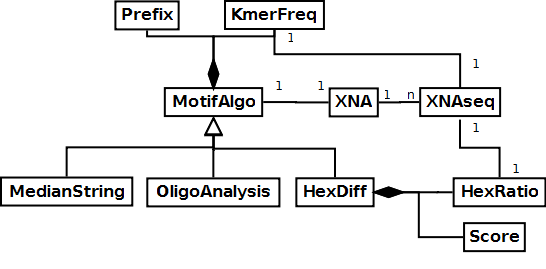
\includegraphics[scale=0.7]{./imagens/MotifAlgo2.png}
    \caption{Diagrama de classes}
    \label{fig:MotifAlgo2}
\end{figure}

As classes responsáveis pela manipulação das sequências são as classes \textbf{DNA} e \textbf{DNAseq} (figura \ref{fig:DNAeDNAseq}). A classe \textbf{DNA} o principal objetivo é manter um conjunto de sequências de DNA, este conjunto é armazenado em um vetor de objetos do tipo \textbf{DNAseq}, as outras funcionalidades dela são: ler um arquivo de sequências do tipo \textit{fasta} (figura \ref{fig:exe_seq}); escrever um arquivo do tipo \textit{fasta} e adicionar uma nova sequência ao conjunto. A classe  \textbf{DNAseq}, foi criada para a manipulação de uma sequência, nela é possível: inserir a sequência, inserir as descrições da sequência e o identificador da mesma. Também é possível gerar o complemento da sequência, o reverso complemento e extrair o tamanho da sequência.


\begin{figure}[htb!]
    \centering
    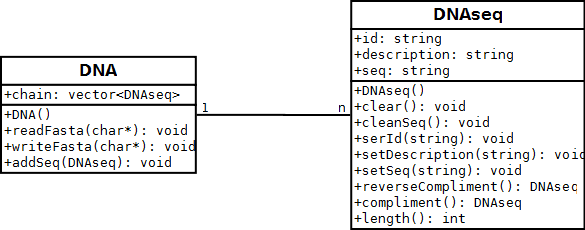
\includegraphics[scale=0.7]{./imagens/DNA.png}
    \caption{Classes DNA e DNAseq}
    \label{fig:DNAeDNAseq}
\end{figure}


\begin{figure}[htb!]
    \centering
    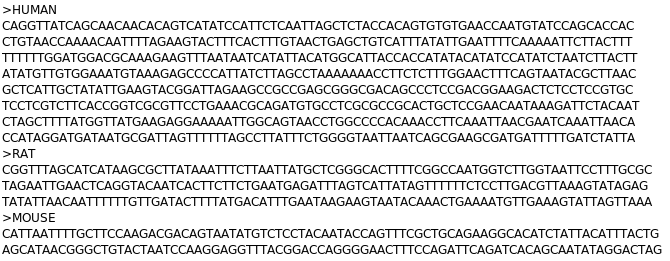
\includegraphics[scale=0.7]{./imagens/exe_seq.png}
    \caption{Exemplo de arquivo \textit{fasta}}
    \label{fig:exe_seq}
\end{figure}

Seguindo temos a classe \textbf{MotifAlgo} (figura \ref{fig:MotifAlgo}), está classe implementa funções que são partilhadas entre as classes que implementam os algoritmos de busca. Nela é possível através do método \textbf{computeTotalFrequency(DNA,int)}, calcular todas as ocorrências e frequências de todos os possíveis oligonucleotídio em uma sequência, o tamanho dos oligonucleotídios é definido no segundo parâmetro do método, a computação das ocorrências dos oligonucleotídios é feita com o auxilio do software Meryl \cite{Walenz:2011:Online}, ele foi utilizado por ser otimizado para este tipo de tarefa, e também mostrou-se mais rápido do que a implementação feita para este propósito. Com o método \textbf{computeMotifFrequency(DNA,DNAseq)}, assim como o método anterior calcula a frequência de oligonucleotídios, a diferença é que ele não calcula para todos os possíveis oligonucleotídios, mas sim para um oligonucleotídio definido pelo usuário. O método \textbf{buildTransitionalTable()}, ele cria uma matriz de transição que é utilizada no modelo de Markov, para criar a matriz este método utiliza as frequências dos oligonucleotídios calculadas, para utiliza-lo é necessário antes rodar o método \textbf{computeTotalFrequency(DNA,int)}, que armazena as frequências na variável \textbf{frequencies} esta variável com todas as frequências é usada então pelo \textbf{buildTransitionalTable()}. Por último temos o método \textbf{scoreSeqMarkov(DNAseq,int)}, ele calcula a probabilidade de um oligonucleotídio aparecer em uma sequência, segundo o  \textit{background} calculado com \textbf{buildTransitionalTable()}.

\begin{figure}[htb!]
    \centering
    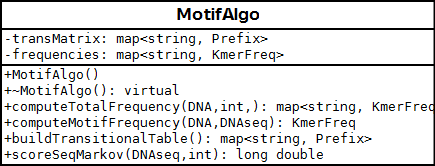
\includegraphics[scale=0.7]{./imagens/MotifAlgo.png}
    \caption{Classe MotifAlgo}
    \label{fig:MotifAlgo}
\end{figure}

As classes \textbf{KmerFreq} e \textbf{Prefix} (figura \ref{fig:KmerPrefix}), atuam como auxiliares da classe \textbf{MotifAlgo}. Um objeto da \textbf{KmerFreq} armazena um oligonucleotídio, as ocorrências deste oligonucleotídio nas sequências e a sua frequência. Um objeto da classe \textbf{Prefix}, é utilizado para armazenar um prefixo de um oligonucleotídio as quatro possibilidades de sufixo (A,C,G,T) e a soma das frequências dos oligonucleotídios formados com a concatenação do prefixos com os sufixos, está classe é utilizada na construção da matriz de transição.

\begin{figure}[htb!]
    \centering
    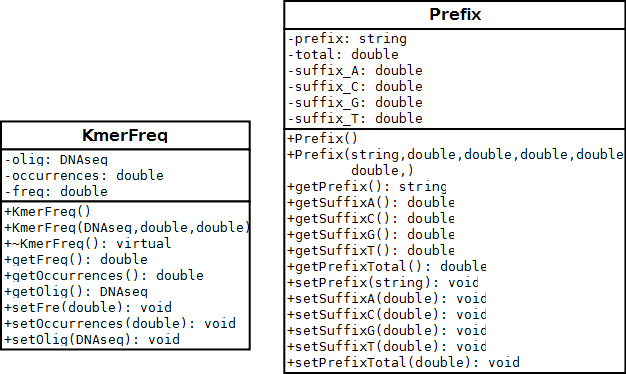
\includegraphics[scale=0.7]{./imagens/KmerPrefix.png}
    \caption{Classes KmerFreq e Prefix}
    \label{fig:KmerPrefix}
\end{figure}


A implementação do algoritmo Median String é feita pela classe \textbf{MedianString} (figura \ref{fig:MedianString}). O principal método é o  \textbf{computeMedianString(DNAseq,int,int)} ele cria a cada rodada um prefixo que começa com apenas uma base e vai incrementando até o tamanho do oligonucleotídio escolhido pelo usuário. Cada prefixo é comparado com todas as sequências procurando a menor distância, isto é feito pelo método \textbf{totalDistance(DNAseq,DNA,int)}, este método percorre todas as sequências e extrai fragmentos da sequência do mesmo tamanho do prefixo, então ele faz uma chamada ao método \textbf{hammingDistance(string,string)}, este retorna a distância entre o prefixo e o fragmento da sequência, as menores distâncias entre as sequências é somada e retornada. O valor da distância do prefixo é comparado com o melhor valor já encontrado (este valor é iniciado com número grande), se a distancia do prefixo for maior, é feita uma chamada ao método \textbf{bypass(DNAseq,int)} que troca por outra a primeira base do prefixo, . Se o valor for menor, é modificado  a última base com o método \textbf{nextVertex(DNAseq,int,int)}. Após ser computada todas as possibilidades para o prefixo, a menor distância encontrada substitui o melhor valor já encontrado, então é incrementado mais uma base ao prefixo, que retorna aos passos anteriores, isto é feito até atingir o tamanho do oligonucleotídio. Ao final o é retornado os oligonucleotídios com as menores distâncias.

\begin{figure}[htb!]
    \centering
    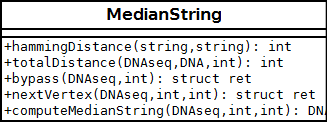
\includegraphics[scale=0.7]{./imagens/MedianString.png}
    \caption{Classe MedianString}
    \label{fig:MedianString}
\end{figure}


A classe \textbf{OligoAnalysis} (figura \ref{fig:OligoAnalysis}) implementa o algoritmo Oligo-Analysis, ela herda os métodos da classe \textbf{MotifAlgo}. O método \textbf{performAnalysis(DNA,double,int)} calcula o complemento reverso de todas as sequências e adiciona no conjunto de sequências, então ele faz uma chamada ao método \textbf{computeTotalFrequency(DNA,int)} para calcular a frequência e aos métodos \textbf{buildTransitionalTable()} e \textbf{scoreSeqMarkov(DNAseq,int)}, o retorno do último método são as sequências esperadas, com elas é calculado a distribuição binomial \textbf{binomialPValue(double,double,double)} as possibilidade de encontrar ocorrer $n$ ou mais oligonucleotídio na sequência \textbf{binomialOccGreater(double,double,double)}, e com o resultado do último método calcular o \textbf{sigValue(double,int)} (valor $sig$).


\begin{figure}[htb!]
    \centering
    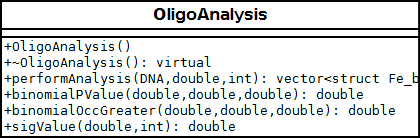
\includegraphics[scale=0.7]{./imagens/OligoAnalysis.png}
    \caption{Classe OligoAnalysis}
    \label{fig:OligoAnalysis}
\end{figure}


O algoritmo HexDiff é implementado pela classe \textbf{HexDiff} (figura \ref{fig:HexDiff}), ela também herda as funcionalidades da classe \textbf{MotifAlgo}. No método \textbf{performFrequency()} é caculado a frequência de todos os possíveis oligonucleotídios de tamanho seis nos dos dados de entrada positivo e negativo, também é calculada a razão, então os oligonucleotídios  e a razão calculada para eles são armazenados em um objeto da classe \textbf{HexRatio}, que é uma classe auxiliar a \textbf{HexDiff} utilizada apenas para este fim. Todos os objetos da classe \textbf{HexRatio} são alocados em um vetor $Hd$, os $n$ oligonucleotídios com maior razão são mantidos no $Hd$ o restante é apagado, isto é feito com o método \textbf{chooseHexamers()}. Por último, com \textbf{computeScore()} é computado a pontuação de todas as possíveis janelas de tamanho de tamanho definido pelo usuário de 1000-2000 pares de bases, as janelas que excederem um limite determinado pelo usuário são consideradas possíveis CRMs, e são alocadas em um vetor de objetos da classe \textbf{Score}, esta classe também é uma auxiliar onde é armazenado a posição da janela encontrada e a pontuação obtida.

\begin{figure}[htb!]
    \centering
    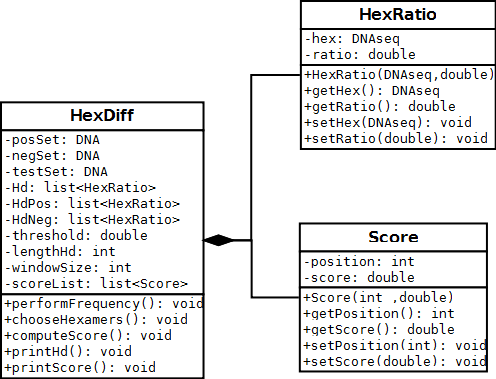
\includegraphics[scale=0.7]{./imagens/HexDiff.png}
    \caption{Classes HexDiff, HexRatio e Score}
    \label{fig:HexDiff}
\end{figure}
